\section{Experimental setup: hardware and software components}
There are only two hardware devices being used in the system: a computing unit and a sensor. 
It was previously explained in section \ref{system_description} that the sensor being used as input of the software is an RGB-D (Red, Green, Blue and Depth) sensor. 
The computing unit used in the experiments is a laptop, whose technical details are presented in section \ref{computer}. 
Those details such as the processor speed and the RAM memory determine the results of the computing performance evaluation experiments. 
\\

In this section the hardware specifications of the hardware used in the experiments is presented. 
It is shown as well the software that is needed to permit the correct functioning of the RGB-D sensor.


% This section shows the hardware specifications with which the testing was performed. 

\subsection{Computer hardware specifications}
\label{computer}
	The computer used for testing the software is a Mountain f-11 Ivy. %, shown in figure \ref{laptop}.
	This laptop has a Intel Core i7-3630QM  CPU that operates at a speed of 2.4 GHz and has the capability of enhancing this speed up to 2.4 GHz. 
	It features a 8 GB Kingston HyperX at 1.600 MHz RAM memory and a  Kingston HyperX 3K of 120 GB Solid State Drive (SSD).
	% \begin{figure}[H]
	% 	\begin{center}
	% 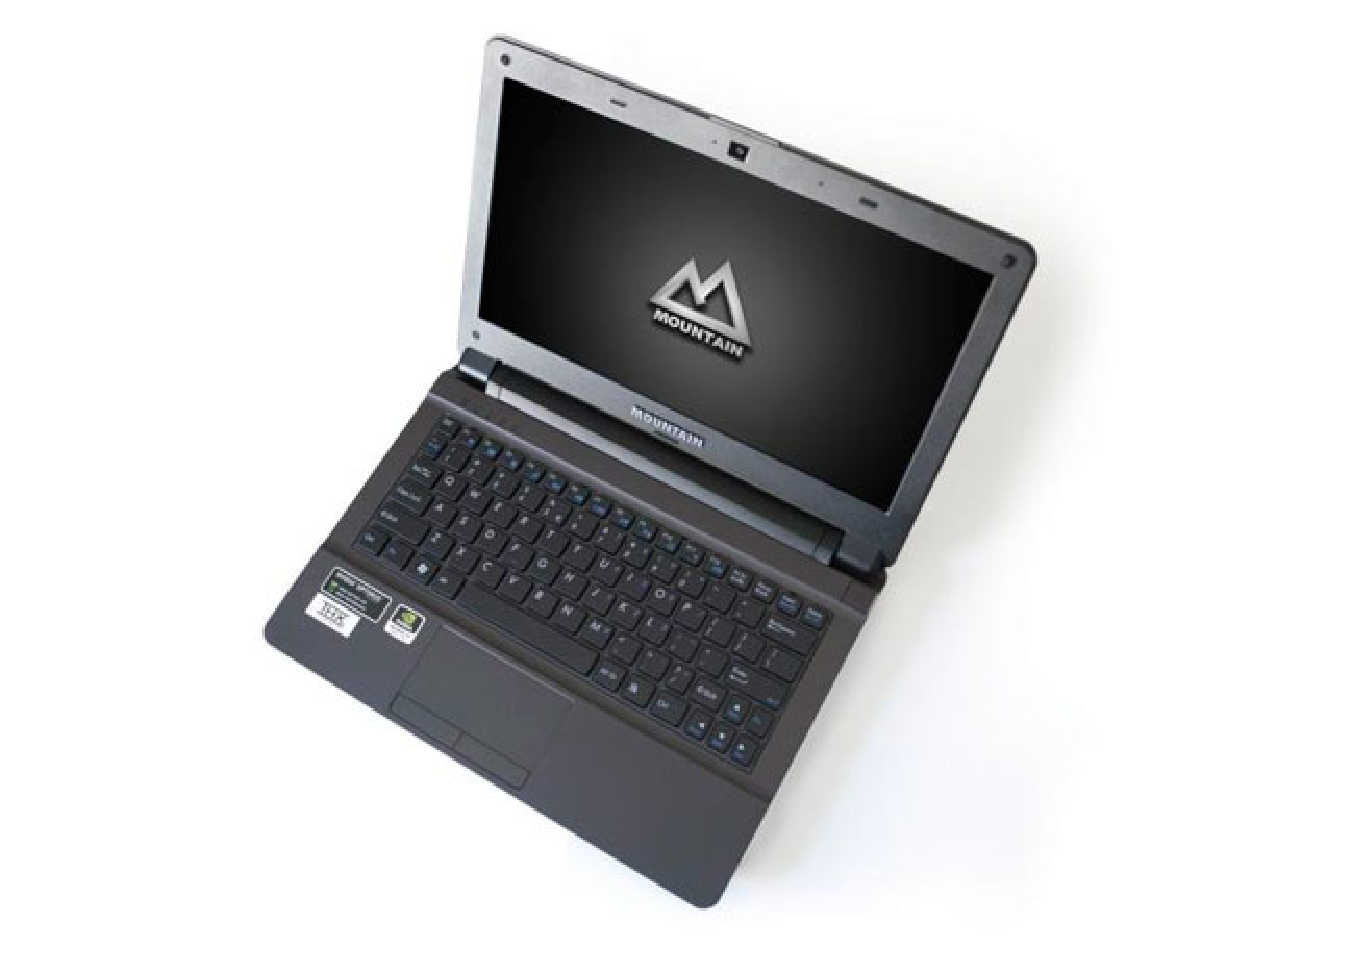
\includegraphics[scale=0.3]{img/mountain.eps}
	% 	\caption[Mountain laptop]{Mountain f-11 Ivy Laptop}
	% 			\label{laptop}

	% 	\end{center}
	% \end{figure}


	% \paragraph{Processing Units} \mbox{}\\
	% 	\begin{itemize}
	% 		\item{CPU: Intel Core i7-3630QM at 2,40 GHz, Turbo Boost up to 3,4 GHz.}
	% 		\item{Integrated GPU:  Intel HD Graphics 4000 at 650 MHz,  Turbo up to 1.1 GHz }
	% 		\item{Dedicated GPU: NVidia GeForce GT 650M with 2 GB of DR3 memory at 835 MHz }
	% 	\end{itemize}

	% 	% \vspace*{0.5cm}

	% \paragraph{Memories} \mbox{}\\
	% 	\begin{itemize}
	% 		\item{RAM : 8 GB Kingston HyperX at 1.600 MHz }
	% 		\item{SSD : Kingston HyperX 3K, 120 GB}
	% 	\end{itemize}
		% \vspace*{0.5cm}

	% \paragraph{Other specifications}
	% 	\begin{itemize}
	% 		\item{Screen: 11.6 '' LED }
	% 		\item{Ports: 3 x USB 3.0 , 1 x USB 2.0 , 1 x HDMI, 1 x VGA, 2 x audio jacks}
	% 		\item{Battery: 6 cells}
	% 		\item{Weight: 1.8kg}
	% 	\end{itemize}
	% 	% \vspace*{0.5cm}

		% \vspace*{0.5cm}

\subsection{RGB-D sensor}
	The RGB-D sensor used in the testing process is a Kinect 360. 
	This sensor is able to retrieve color and depth information using its color and depth-sensing lenses. 
	These lenses determine the field of view of the sensor as well as its working depth range. 
	The horizontal field of view is 57 degrees and the vertical field of view, 43 degrees. 
	The kinect is able to work correctly between 1.2 m and 3.5 m, which is the maximum depth sensor range. 
	\\

	The sensor outputs two data streams, one containing the depth information and the other containing the color data. 
	The first one is a matrix of 320x240 of 16-bit information that is outputted at a rate of 30 frames per second. 
	The color information is a matrix of 640x480 composed of 32-bit data that is published at a rate of 30 frames per second as well. 

	% Figure \ref{kinect_image} shows its external appearance. 
	% Its technical details are the following: 
	% \begin{figure}[H]
	% 	\begin{center}
	% 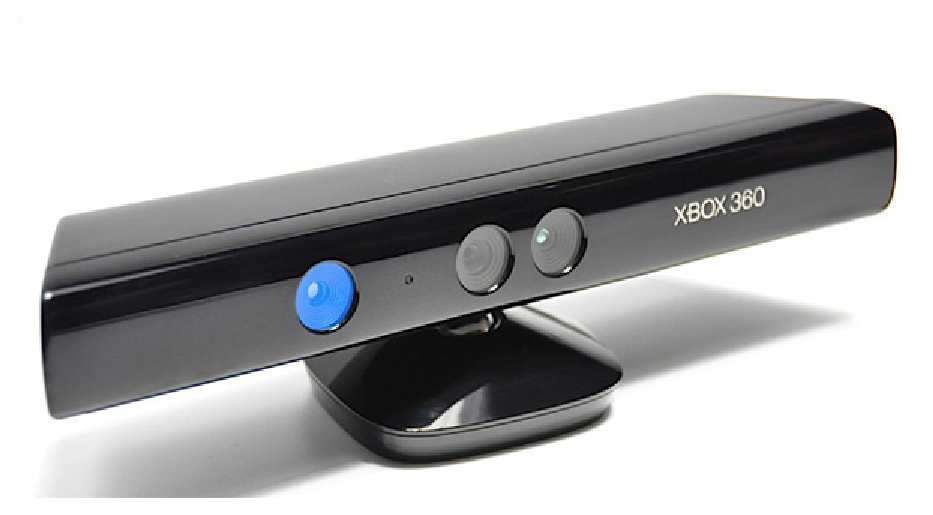
\includegraphics[scale=0.3]{img/kinect.eps}
	% 	\caption[Kinect image]{Kinect for XBOX 360}
	% 		\label{kinect_image}

	% 	\end{center}
	% \end{figure}
% 	\paragraph{ Sensor} \mbox{} \\
% 		\begin{itemize}
% 			\item Colour and depth-sensing lenses
% 			% \item Voice microphone array
% 			% \item Tilt motor for sensor adjustment
% 			% \item Fully compatible with existing Xbox 360 consoles
% 		\end{itemize}
% %		\vspace*{0.5cm}

% 	\paragraph{ Field of View} \mbox{} \\
% 		\begin{itemize}

% 			\item Horizontal field of view: 57 degrees
% 			\item Vertical field of view: 43 degrees
% 			\item Physical tilt range: ± 27 degrees
% 			\item Depth sensor range: 1.2m - 3.5m
% 		\end{itemize}
% 		% \vspace*{0.5cm}

% 	\paragraph{ Data Streams} \mbox{} \\
% 		\begin{itemize}

% 			\item 320x240 16-bit depth @ 30 frames/sec
% 			\item 640x480 32-bit colour@ 30 frames/sec
% 			% \item 16-bit audio @ 16 kHz
% 		\end{itemize}
% 		% \vspace*{0.5cm}


	\subsection{Software}
		\begin{itemize}
			\item{OS: Ubuntu 13.04, 64 bits}
			\item{Drivers: OpenNI SDK v1.5.4.0, 64bits}
			\item{Drivers: Avin2-v0.93-5.1.2.1}
			\item{Drivers: NITE v1.5.2.21, 64 bits}
			\item{ROS Groovy}
			\item{OpenCV: }
			\item{PCL : }
			\item{openni\_camera}
			\item{openni\_launch}
			\item{pi\_tracker}


		\end{itemize}